% !TEX TS-program = knitr
\documentclass{article}\usepackage{graphicx, color}
%% maxwidth is the original width if it is less than linewidth
%% otherwise use linewidth (to make sure the graphics do not exceed the margin)
\makeatletter
\def\maxwidth{ %
  \ifdim\Gin@nat@width>\linewidth
    \linewidth
  \else
    \Gin@nat@width
  \fi
}
\makeatother

\IfFileExists{upquote.sty}{\usepackage{upquote}}{}
\definecolor{fgcolor}{rgb}{0.2, 0.2, 0.2}
\newcommand{\hlnumber}[1]{\textcolor[rgb]{0,0,0}{#1}}%
\newcommand{\hlfunctioncall}[1]{\textcolor[rgb]{0.501960784313725,0,0.329411764705882}{\textbf{#1}}}%
\newcommand{\hlstring}[1]{\textcolor[rgb]{0.6,0.6,1}{#1}}%
\newcommand{\hlkeyword}[1]{\textcolor[rgb]{0,0,0}{\textbf{#1}}}%
\newcommand{\hlargument}[1]{\textcolor[rgb]{0.690196078431373,0.250980392156863,0.0196078431372549}{#1}}%
\newcommand{\hlcomment}[1]{\textcolor[rgb]{0.180392156862745,0.6,0.341176470588235}{#1}}%
\newcommand{\hlroxygencomment}[1]{\textcolor[rgb]{0.43921568627451,0.47843137254902,0.701960784313725}{#1}}%
\newcommand{\hlformalargs}[1]{\textcolor[rgb]{0.690196078431373,0.250980392156863,0.0196078431372549}{#1}}%
\newcommand{\hleqformalargs}[1]{\textcolor[rgb]{0.690196078431373,0.250980392156863,0.0196078431372549}{#1}}%
\newcommand{\hlassignement}[1]{\textcolor[rgb]{0,0,0}{\textbf{#1}}}%
\newcommand{\hlpackage}[1]{\textcolor[rgb]{0.588235294117647,0.709803921568627,0.145098039215686}{#1}}%
\newcommand{\hlslot}[1]{\textit{#1}}%
\newcommand{\hlsymbol}[1]{\textcolor[rgb]{0,0,0}{#1}}%
\newcommand{\hlprompt}[1]{\textcolor[rgb]{0.2,0.2,0.2}{#1}}%

\usepackage{framed}
\makeatletter
\newenvironment{kframe}{%
 \def\at@end@of@kframe{}%
 \ifinner\ifhmode%
  \def\at@end@of@kframe{\end{minipage}}%
  \begin{minipage}{\columnwidth}%
 \fi\fi%
 \def\FrameCommand##1{\hskip\@totalleftmargin \hskip-\fboxsep
 \colorbox{shadecolor}{##1}\hskip-\fboxsep
     % There is no \\@totalrightmargin, so:
     \hskip-\linewidth \hskip-\@totalleftmargin \hskip\columnwidth}%
 \MakeFramed {\advance\hsize-\width
   \@totalleftmargin\z@ \linewidth\hsize
   \@setminipage}}%
 {\par\unskip\endMakeFramed%
 \at@end@of@kframe}
\makeatother

\definecolor{shadecolor}{rgb}{.97, .97, .97}
\definecolor{messagecolor}{rgb}{0, 0, 0}
\definecolor{warningcolor}{rgb}{1, 0, 1}
\definecolor{errorcolor}{rgb}{1, 0, 0}
\newenvironment{knitrout}{}{} % an empty environment to be redefined in TeX

\usepackage{alltt}

\usepackage{amsfonts}
\usepackage{amsmath}
\usepackage{amssymb}
\usepackage{amsthm}
\usepackage{caption}
\usepackage{color}
\usepackage{enumerate}
\usepackage{fancyhdr}
\usepackage{hyperref}
\usepackage{graphicx}
\usepackage{latexsym}
\usepackage{listings}
\usepackage{mathrsfs}
\usepackage{natbib}
\usepackage[nottoc]{tocbibind}
\usepackage{url}

\providecommand{\all}{\ \forall \ }
\providecommand{\bs}{\backslash}
\providecommand{\e}{\varepsilon}
\providecommand{\E}{\ \exists \ }
\providecommand{\lm}[2]{\lim_{#1 \rightarrow #2}}
\providecommand{\m}[1]{\mathbb{#1}}
\providecommand{\nv}{{}^{-1}}
\providecommand{\ov}[1]{\overline{#1}}
\providecommand{\p}{\newpage}
\providecommand{\q}{$\quad$ \newline}
\providecommand{\rt}{\rightarrow}
\providecommand{\Rt}{\Rightarrow}
\providecommand{\vc}[1]{\boldsymbol{#1}}
\providecommand{\wh}[1]{\widehat{#1}}

%\renewcommand\bibname{References}
%\renewcommand{\thesection}{Problem \arabic{section}}
%\renewcommand{\thesubsection}{Part \alph{subsection}}
\numberwithin{equation}{section}

\fancyhead{}
\fancyfoot{}
\fancyhead[R]{\thepage}
\fancyhead[C]{Landau}

\hypersetup{
    colorlinks,
    citecolor=black,
    filecolor=black,
    linkcolor=black,
    urlcolor=blue
}

\definecolor{dkgreen}{rgb}{0,0.6,0}
\definecolor{gray}{rgb}{0.5,0.5,0.5}
\definecolor{mauve}{rgb}{0.58,0,0.82}

\lstset{ 
  language=C,                % the language of the code
  basicstyle=\Large,           % the size of the fonts that are used for the code
  numberstyle= \tiny \color{white},  % the style that is used for the line-numbers
  stepnumber=2,                   % the step between two line-numbers. 
  numbersep=5pt,                  % how far the line-numbers are from the code
  backgroundcolor=\color{white},      % choose the background color. You must add \usepackage{color}
  showspaces=false,               % show spaces adding particular underscores
  showstringspaces=false,         % underline spaces within strings
  showtabs=false,                 % show tabs within strings adding particular underscores
  frame=lrb,                   % adds a frame around the code
  rulecolor=\color{black},        % if not set, the frame-color may be changed on line-breaks within not-black text 
  tabsize=2,                      % sets default tabsize to 2 spaces
  captionpos=t,                   % sets the caption-position 
  breaklines=true,                % sets automatic line breaking
  breakatwhitespace=false,        % sets if automatic breaks should only happen at whitespace
  title=\lstname,                   % show the filename of files included with \lstinputlisting;
  keywordstyle=\color{blue},          % keyword style
  commentstyle=\color{gray},       % comment style
  stringstyle=\color{dkgreen},         % string literal style
  escapeinside={\%*}{*)},            % if you want to add LaTeX within your code
  morekeywords={*, ...},               % if you want to add more keywords to the set
  xleftmargin=0.053in, % left horizontal offset of caption box
  xrightmargin=-.03in % right horizontal offset of caption box
}

\DeclareCaptionFont{white}{\color{white}}
\DeclareCaptionFormat{listing}{\parbox{\textwidth}{\colorbox{gray}{\parbox{\textwidth}{#1#2#3}}\vskip-0.05in}}
\captionsetup[lstlisting]{format = listing, labelfont = white, textfont = white}
% For caption-free listings, comment out the 3 lines above and uncomment the 2 lines below.
% \captionsetup{labelformat = empty, labelsep = none}
% \lstset{frame = single}






\begin{document}



\begin{flushleft}


\begin{center} \LARGE
STAT 305 D Homework 3 
\end{center}
\begin{center} \Large
Due February 7, 2012 at 12:40 PM in class
\end{center}


\begin{enumerate}[1. ]

\item Here is dataset giving the number of printer jams per day of a receipt printer in a supermarket for 17 days.





\begin{align*}
43,100, 500,23,89,89,89,89,72,72,72,21,32,41,39,47,56
\end{align*} 

\begin{itemize}
\item Identify the sample.
\item Identify the population.
\item Calculate the sample mean.
\item Calculate the median.
\item Calculate the mode.
\item Calculate the sample variance.
\item Calculate the sample standard deviation.
\item Calculate the range.
\end{itemize}


\item Chapter 3 section 2 part of exercise 1 (page 92): 

\setkeys{Gin}{width=.75\textwidth} 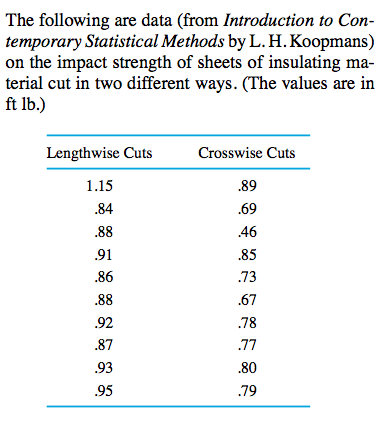
\includegraphics{../../fig/ch3s2p1.png}




For the lengthwise sample, $Q(0.25) = 0.870, Q(0.5) = 0.895$, and $Q(0.75) = 0.930$. For the crosswise sample, $Q(0.25) = 0.690, Q(0.5) =0.775$, and $Q(0.75) = 0.800$. 

\begin{enumerate}[a. ]
\item Find the IQR.
\item Draw (to scale) carefully labeled side-by-side boxplots for comparing the two
cutting methods. Discuss what these show about the two methods.
\item Make and discuss the appearance of a Q-Q (quantile-quantile) plot for comparing
the shapes of these two data sets.
\end{enumerate}



\item Below is a normal quantile plot of the yield data from problem 1 (Chapter 3 Section 1 Exercise 1, page 77). What does this plot tell you about the distributional shape of the yield data? Justify your answer based on the shape of the points in the plot.

\setkeys{Gin}{width=1\textwidth} 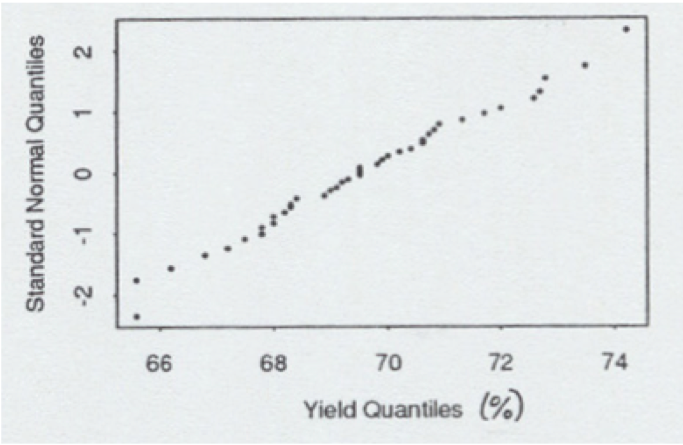
\includegraphics{../../fig/ch3s1p1c2.png}











\item You work for one of the main manufactures of fire rescue harnesses in the United States. In the news one day, you read about a firefighter who was using one of your company�s harnesses in a rescue and suffered an accident because a clasp on his harness came undone. You contact the firefighter, obtain the harness that failed, and determine that the bad clasp was originally faulty when it came out of the plant in Gary, IN. Concerned that other harnesses may have faulty clasps, you consult your supervisor. He informs you that he is already investigating the problem, and he shows you the following bar chart:

\setkeys{Gin}{width=1\textwidth} 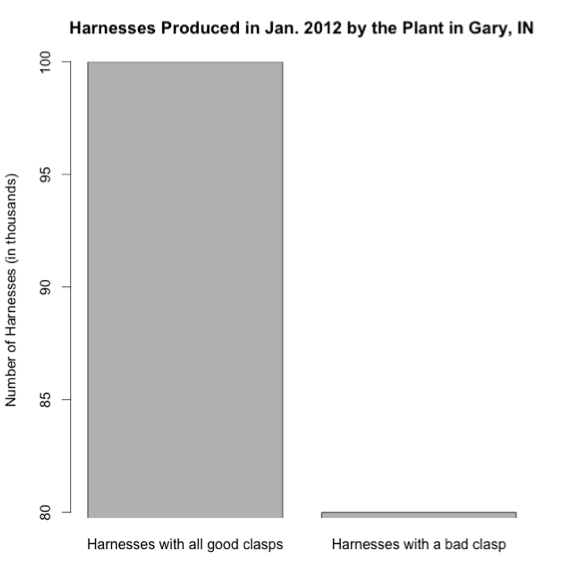
\includegraphics{../../fig/harnesses.png}

\begin{enumerate}[1. ]
\item Is the above plot an honest representation of the data? Why or why not? If there is there anything misleading about the plot, what is it?
\item Should the company arrange a recall of the harnesses produced in Jan. 2012 by the Gary plant, or is a recall unnecessary?
\end{enumerate}




\item Vardeman and Jobe chapter 4 section 1 problem 3 parts a-c (page 140). Data can be found at \url{http://www.will-landau.com/stat305/data/csv/polypolyols.csv}.You're welcome to use a spreadsheet program to do this problem, but please show your calculations. If you use Excel formulas, for example, please write them down. The article �Polyglycol Modified Poly (Ethylene Ether Carbonate) Polyols by Molecular Weight Advancement� by R. Harris (Journal of Applied Poly- mer Science, 1990) contains some data on the effect of reaction temperature on the molecular weight of resulting poly polyols. The data for eight experimental runs at temperatures 165${}^\circ$C and above are as follows. Here, $x$ is pot temperature (${}^\circ$) and $y$ is average molecular weight.


% latex table generated in R 2.15.1 by xtable 1.7-0 package
% Sun Feb 17 16:51:26 2013
\begin{table}[ht]
\begin{center}
\begin{tabular}{rr}
 x & y \\ 
  \hline
165.00 & 808.00 \\ 
  176.00 & 940.00 \\ 
  188.00 & 1183.00 \\ 
  205.00 & 1545.00 \\ 
  220.00 & 2012.00 \\ 
  235.00 & 2362.00 \\ 
  250.00 & 2742.00 \\ 
  260.00 & 2935.00 \\ 
  \end{tabular}
\end{center}
\end{table}




\begin{enumerate}[a. ]
\item What fraction of the observed raw variation in
y is accounted for by a linear equation in x?
\item Fit a linear relationship $y \approx b_0 + b_1 x$ to these data via least squares. About what change in average molecular weight seems to accompany a $1^\circ C$ increase in pot temperature (at least over the experimental range of temperatures)?
\item Compute and plot residuals from the linear relationship fit in (b). Discuss what they suggest about the appropriateness of that fitted equation. (Plot residuals versus $x$ and residuals versus $\wh{y}$.)
\end{enumerate}






\item Vardeman and Jobe chapter 4 section 1 problem 4 (page 140). Data can be found at \url{http://www.will-landau.com/stat305/data/csv/tools.csv}.

\setkeys{Gin}{width=.75\textwidth} 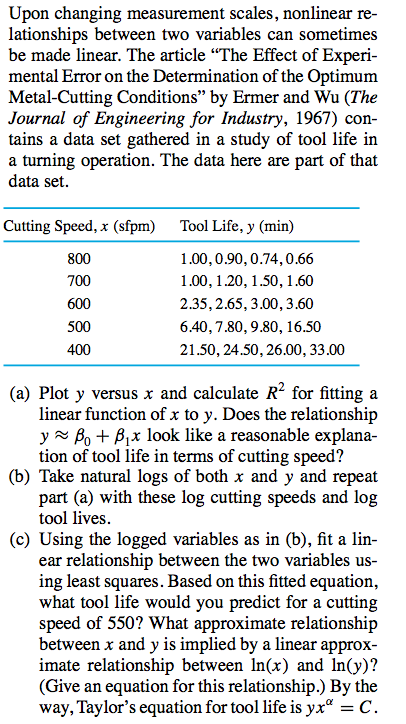
\includegraphics{../../fig/ch4s1p4.png}










\item Weekly feedback. You get full credit as long as you write something.
\begin{enumerate}[1. ]
\item Is there any aspect of the subject matter that you currently struggle with? If so, what specifically do you find difficult or confusing? The more detailed you are, the better I can help you.
\item Do you have any questions or concerns about the material, class logistics, or anything else? If so, fire away.
\end{enumerate}


\item EXTRA CREDIT. Using the normal quantile plot below, draw the approximate distributional shape of the original data. 

\begin{knitrout}
\definecolor{shadecolor}{rgb}{0.969, 0.969, 0.969}\color{fgcolor}\includegraphics[width=\textwidth]{figure/unnamed-chunk-4} 
\end{knitrout}





\end{enumerate}




\end{flushleft}
%\newpage 
%\nocite{*}
%\bibliographystyle{plainnat} 
%\bibliography{}
\end{document}
